\section{Overview：系统概览}
\sectionen{A shared model, a complete plan, and coordinated execution}

PDblend 的目标，是在满足响应延迟要求的前提下，减少大语言模型推理的 GPU 能量开销。它不要求所有请求都分离：系统比较不同执行方式的成本，决定什么时候启用 P/D、哪些请求进入分离路径，以及给各条路径分配多少资源。本文按三个技术模块解释这一方法：离线性能与能耗建模、选择性分离规划、在线协同与分流。
\EN{PDblend aims to reduce GPU energy while meeting serving-latency targets. It does not disaggregate every request. Instead, it compares execution costs and decides when to use separate prefill and decode pools, which requests should use them, and how much capacity each path receives. Three modules provide the model, choose a complete plan, and carry it out online.}

\paragraph{先理解 P、D 和 M。}
P（prefill）读取输入并建立 KV 缓存；在本文的接力协议中，它还产生首个输出 token。D（decode）利用已有缓存，继续生成后续 token。M（mixed）在同一个实例内完成这两个阶段。token 是模型处理的文本片段，不一定等于一个汉字；KV 则是后续生成可以复用的中间状态。
\EN{Prefill, denoted P, processes the prompt and creates its KV state; the carry protocol also obtains the first output token from P. Decode, denoted D, reuses this state to generate subsequent tokens. A mixed instance, M, performs both stages locally. Tokens are model text units, and KV is reusable intermediate state.}

\begin{figure*}[t]
  \centering
  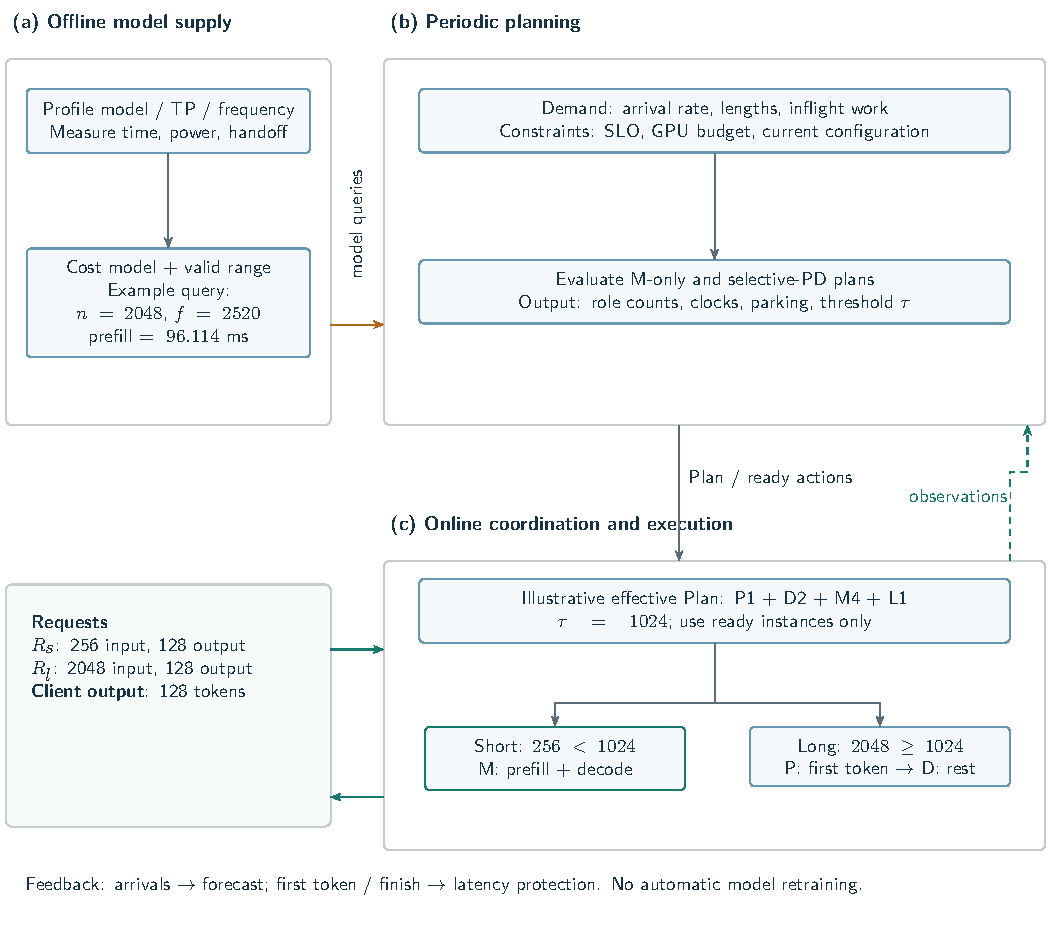
\includegraphics[width=\textwidth]{figures/01-overview.pdf}
  \caption{三个模块通过模型查询、完整 Plan 和在线观测形成闭环。图中的八实例配置与请求是协作机制示例，不是某次最优规划的测量结果。实线区分模型供给与执行流，虚线为观测反馈。\newline
  Three modules exchange model queries, complete plans, and online observations. The eight-instance layout and requests illustrate coordination, not a measured optimal plan. Dashed arrows carry feedback; the offline model is not automatically retrained by this loop.}
  \label{fig:overview}
\end{figure*}

\paragraph{为什么需要选择性分离。}
在 M 上执行可以省去跨实例交接，但较长的 prefill 可能拖慢同机的 decode。分离后，P 和 D 可以各自配置资源与频率，却要付出 KV 交接、调度以及维持不同资源池的代价。因此，长请求并非总应分离，短请求也不能仅凭长度忽略系统状态；决策要同时看负载、延迟和完整成本。
\EN{Mixed execution avoids an inter-instance handoff, but long prefills can interfere with ongoing decoding. Separate pools allow different allocations and clocks, at the cost of KV transfer, coordination, and pool capacity. Length is therefore a routing signal within a workload-aware plan, rather than a universal rule that long requests must always be separated.}

\begin{table}[t]
  \centering\small
  \caption{模块接口 / Module interfaces}
  \label{tab:interfaces}
  \begin{tabularx}{\columnwidth}{@{}p{.18\columnwidth}XX@{}}
    \toprule
    模块 & 输入 / Input & 输出 / Output\\
    \midrule
    建模 & 模型、硬件、并行配置、样本 & 时间、功率、开销与有效范围\\
    规划 & 模型、负载、SLO、预算、当前配置 & 角色数、频率、停驻状态、阈值\\
    在线 & 请求、Plan、负载与执行状态 & token、有效配置、动作与反馈\\
    \bottomrule
  \end{tabularx}
\end{table}

\paragraph{三个模块的职责。}
离线模块回答“一个候选方案大概花多少时间、消耗多少能量”，不直接决定请求去向。规划模块把请求到达率和长度分布转为两条路径的负载，比较候选方案，输出一份完整 Plan。在线模块把 Plan 落实到就绪实例，并持续收集观测；有风险时，快速保护可以提前触发新一轮规划。
\EN{The model estimates candidate costs without routing requests. The planner translates demand and length statistics into the work assigned to each path, compares candidates, and emits a complete Plan. The runtime applies the Plan to ready instances and reports observations. Protection can request replanning before the next periodic deadline.}

\paragraph{Plan 为什么必须完整。}
一个阈值无法独立描述分离方案。阈值改变后，两边需要的容量也会改变。因此，Plan 一起指定 P/D/M 实例数、各池频率、停驻状态与长度阈值。新阈值只有在对应路径容量就绪后才能生效。已开始执行的请求保持自己的路径，不能因下一轮计划改变而被悄悄迁移。
\EN{A threshold alone does not define a disaggregated configuration: moving requests changes the capacity each path needs. A Plan therefore binds role counts, clocks, parking states, and the threshold. A new threshold becomes effective with sufficient ready path capacity. Ongoing requests retain their execution ownership across plan changes.}

\paragraph{统一的请求规格，不混淆各图假设。}
下文使用 8 个 TP1 实例，每个实例占一张 GPU。短输入为 256 或 512 token，长输入为 2048 或 4096 token，输出预算均为 128。阈值示例为 1024。图~\ref{fig:planning}演算三个候选的比较规则；图~\ref{fig:routing}另用一份已生效的 PD 配置解释执行，不把后者当作前者的最终输出。
\EN{Examples share eight TP1 instances, one GPU per instance, prompt lengths of 256, 512, 2048, or 4096 tokens, and an output budget of 128. A threshold of 1024 separates the prompt groups. Figure~\ref{fig:planning} examines selected candidates; Figure~\ref{fig:routing} uses a separate effective PD layout to explain execution. Their configuration assumptions are stated independently.}

\paragraph{怎样读延迟与能量。}
TTFT 是从请求提交到客户端收到首个 token 的时间；TPOT 是首 token 之后生成一个 token 的平均耗时。SLO 是对这些延迟的服务目标。本文能量范围为指定 GPU 的板卡能量，包含仍有静态功率的停驻或关闭实例，不等于主机整机能量。模型预测、合成例子与硬件实测需要分别标注。
\EN{TTFT ends when the client receives the first token. TPOT describes the mean time per subsequent output token. SLOs specify the latency targets. Energy covers the selected GPU boards, including inactive devices with nonzero static draw; it is not whole-host energy. Model estimates, synthetic demonstrations, and hardware measurements remain distinct.}

\paragraph{本文的设计口径。}
正文描述目标 selective PD 设计，各技术章末用短注说明当前实现差异。数值查询统一来自仓库的合成测试模型，可由附带脚本复算；该模型直接构造系数，不能充当真实采样、拟合精度或正式评测通过的证据。详细源代码版本、计算输出和构建依赖随源码包保存。
\EN{The main text describes the target selective-PD design; implementation notes identify current gaps. Numeric queries use one reproducible synthetic fixture whose coefficients are constructed directly. It provides no evidence of hardware profiling accuracy or formal acceptance. Source identities, calculations, and build dependencies accompany the editable paper.}
